\documentclass{article}

\usepackage{graphicx}

\begin{document}
	\section*{Lab3 - Filip Jędrzejewski}
	
	\subsection*{Opis problemu}
	
	Populacja Stanow zjednoczonych na przestrzeni lat przedstawiala sie nastepujaco:
	
	\begin{center}
		\begin{tabular}{c|c}
  			\hline 
  			Rok & Populacja\\
  			\hline
  			1900 & 76 212 168 \\
  			1910 & 92 228 496 \\
  			1920 & 106 021 537 \\
  			1930 & 123 202 624 \\
  			1940 & 132 164 569 \\
  			1950 & 151 325 798 \\
  			1960 & 179 323 175 \\
  			1970 & 203 302 031 \\
  			1980 & 226 542 199 \\
		\end{tabular} 
		
	\end{center}
	
	W celu wyznaczenia wielomianu, ktory interpoluje powyzsze dziewiec punktow rozwazono nastepujace zbiory funkcji bazowych $\phi (t)$, $j=1,2,...,9$:
	
	\begin{equation}
		\phi_j (t) = t^{j-1}
	\end{equation}
	
	\begin{equation}
		\phi_j (t) = (t-1900)^{j-1}
	\end{equation}
	
	\begin{equation}
		\phi_j (t) = (t-1940)^{j-1}
	\end{equation}
	
	\begin{equation}
		\phi_j (t) = \left(\frac{t-1940}{40}\right)^{j-1}
	\end{equation}
	
	\subsection*{Wyznaczanie wielomianu za pomoca macierzy}
	
	Dla kazdego z czterech zbiorow funkcji bazowych utworzono macierz Vandermonde'a, a nastepnie korzystajac z funkcji \texttt{numpy.linalg.cond} obliczono wspolczynniki uwarunkowania kazdej z nich. Wyniki przedstawiono w tabeli: 
	
	\begin{center}
		\caption{Wspolczynniki uwarunkowania macierzy}
		\begin{tabular}{|c|c|}
  			\hline 
  			Numer funkcji bazowej & Wspolczynnik uwarunkowania macierzy\\
  			\hline
  			1 & $5.031 \cdot 10^{26}$ \\
  			2 & $6.307 \cdot 10^{15}$ \\
  			3 & $9.316 \cdot 10^{12}$ \\
  			4 & $1.605 \cdot 10^{3}$ \\
  			\hline
		\end{tabular} 
		
	\end{center}
	
	Najmniejszy wspolczynnik uwarunkowania miala baza okreslona wzorem (4), zatem zostala ona wybrana do wynaczenia wielomianu interpolacyjnego. W tym celu rozwiazano nastepujace rownanie macierzowe:
	
	\begin{equation}
		M \cdot C = Y
	\end{equation}
	
	przy czym: $M$ - macierz Vandermonde'a utworzona na najlepiej uwarunkowanej bazie, $C$ - szukana macierz wspolczynnikow, $Y$ - macierz wartosci wielomianu dla danych punktow. \\
	Do rozwiazania tego rownania uzyto funkcji \texttt{numpy.linalg.solve}, ktora zwraca rozwiazanie rownania macierzowego typu $AX=B$, gdzie $A$ i $B$ sa dane, a $X$ szukana. \\
	W kolejnym kroku utworzono wykres otrzymanego wielomianu na przedziale $year \in [1900, 1990]$, na który naniesiono wezly interpolacji.
	
	
	\begin{figure}[h]
    		\centering
  		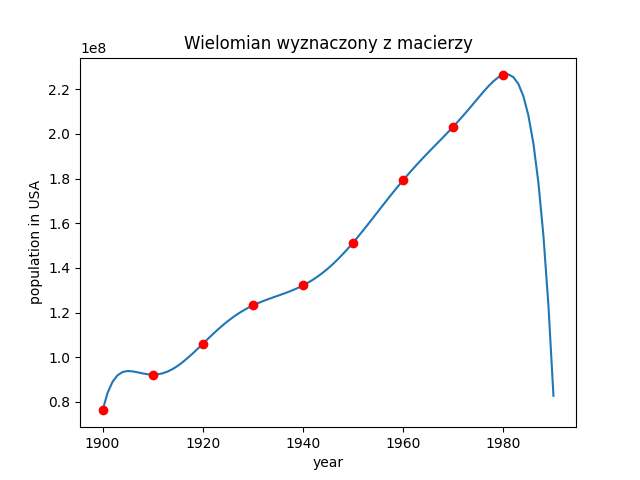
\includegraphics[scale = 0.9]{wykres1.png}
	\end{figure}
	
	Wykres wielomianu interpolacyjnego przechodzi przez wszystkie dziewiec wezlow interpolacji, co potwierdza poprawnosc wykonanej interpolacji.\\
	Kolejna czynnoscia bylo dokonanie ekstrapolacji wielomianu do 1990 roku. Otrzymano wartosc $82749141$, która w porównaniu prawdziwej wartosci populacji dla Stanow Zjednoczonych w 1990 roku, rownej $248709873$, miala blad wzgledny ekstrapolacji rowny:
	
	\begin{equation}
		relativeExtrapolationError = 0.6672864651416437 \approx 66.73 \%
	\end{equation}
	
	
	
	\subsection*{Wyznaczanie wielomianu Lagrange'a}
	
	W celu wyznaczenia wielomianu interpolacyjnego Lagrange'a uzyto nastepujacych wzorow:
	
	\begin{equation}
		l_j (t) = \prod _{k=1, k \neq j} ^ n \frac{t-t_k}{t_j - t_k}
	\end{equation}
	
	\begin{equation}
		p (t) = \sum _{i=1} ^n y_i  l_i(t)
	\end{equation}
	
	Na ich podstawie, korzystajac z funkcji \texttt{lambda}, wyznaczono wielomian interpolacyjny Lagrange'a. Nastepnie obliczono wartosci tego wielomianu dla takiego samego przedzialu jak w poprzednim podpunkcie z krokiem co jeden rok. Na podstawie uzyskanych wartosci stworzono wykres:
	
	\begin{figure}[h]
    		\centering
  		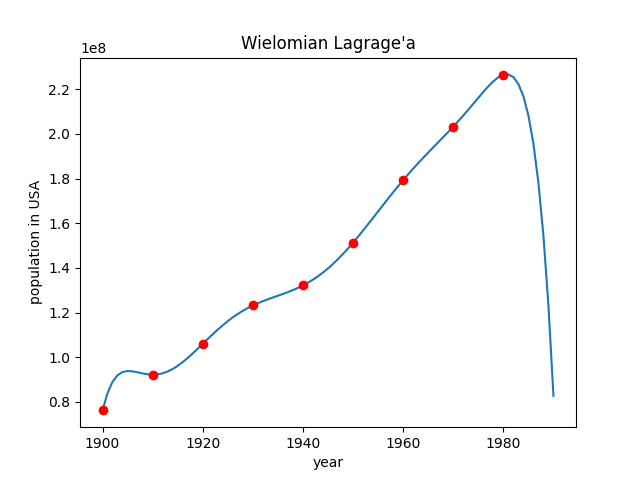
\includegraphics[scale = 0.9]{wykres2.png}
	\end{figure}
	
	Powyzszy wykres jest identyczny jak ten stworzony na podstawie macierzy, co potwierdza poprawnosc wyznaczenia wielomianu metoda Lagrange'a.
	
	
	\subsection*{Wyznaczanie wielomianu Newtona}
	
	W celu wyznaczenia wielomianu interpolacyjnego Newtona uzyto nastepujacych wzorow:
	
	\begin{equation}
		\pi (t) = \prod _{k=1} ^ {j-1} (t-t_k)
	\end{equation}
	
	\begin{equation}
		p (t) = \sum _{i=1} ^n f[t_1,...,t_i] \cdot \pi_i(t)
	\end{equation}
	
	\begin{equation}
		f[x_i] = f(x_i)
	\end{equation}
	
	\begin{equation}
		f[x_i, x_{i+1}] = \frac{f[x_{i+1}]-f[x_{i}]}{x_{i+1} - x_{i}}
	\end{equation}
	
	\begin{equation}
		f[x_0, ..., x_i] = \frac{f[x_1, ..., x_i] - f[x_0,...,x_{i-1}]}{x_i - x_0}
	\end{equation}
	
	Na ich podstawie, korzystajac z funkcji \texttt{lambda} oraz rekurencyjnie obliczajac wartosci ilorazow roznicowych, wyznaczono wielomian interpolacyjny Newtona. Nastepnie obliczono wartosci tego wielomianu dla takiego samego przedzialu jak w pierwszym podpunkcie z krokiem co jeden rok. Na podstawie uzyskanych wartosci stworzono wykres:
	
	\newpage
	
	\begin{figure}[h]
    		\centering
  		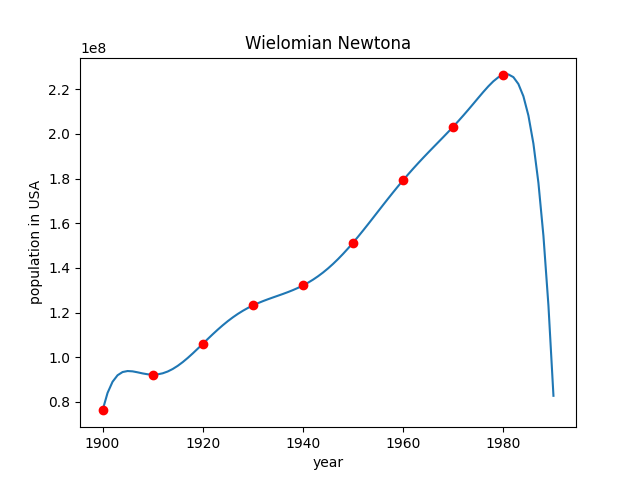
\includegraphics[scale = 0.9]{wykres3.png}
	\end{figure}
	
	Powyzszy wykres jest identyczny jak ten stworzony na podstawie macierzy oraz metoda Lagrange'a, co potwierdza poprawnosc wyznaczenia wielomianu metoda Newtona.
	
	
	
	
	
	
	
	
	
	
	
	
	
	
	
	
	
	
	
	
	
	
	
	
	
	
	
	
	
	
\end{document}